\documentclass{article}
\usepackage{graphicx}
\usepackage{amssymb}
\usepackage{amsmath}
\usepackage{parskip}
\usepackage{tabularray}
\usepackage[a4paper,margin=1.25cm]{geometry}

\newcounter{problem}
\newcounter{extraproblem}
\newcommand{\question}[1]{\refstepcounter{problem}\par\smallskip\textbf{T\theproblem.}\quad #1\par\smallskip}
\newcommand{\extraquestion}[1]{\refstepcounter{extraproblem}\par\smallskip\textbf{OT\theextraproblem.}\quad #1\par\smallskip}

\begin{document}
\title{Homework 1 Clustering and Regression}
\author{Nipat Chenthanakij 6430215121}
\date{}
\maketitle
\subsection*{Metrics}
\begin{center}
    \begin{tblr}{hlines,vlines}
        Model A    & Predicted dog & Predictted cat \\
        Actual dog & 30            & 20             \\
        Actual cat & 10            & 40
    \end{tblr}
\end{center}

\question{What is the accuracy of Model A?}
Accuracy = \(\dfrac{TP+TN}{TP+TN+FP+FN} = \dfrac{30+40}{30+40+10+20}=0.7\)

\question{Consider cats as `class 1' (positive) and dogs as `class 0' (negative). Calculate the precision, recall, and F1.}
Precision = \(\dfrac{TP}{TP+FP} = \dfrac{40}{20+40} = 0.67\)

Recall = \(\dfrac{TP}{TP+FN} = \dfrac{40}{10+40} = 0.8\)

F1 = \(2 \times \dfrac{\text{precision} \times \text{recall}}{\text{precision} + \text{recall}} = 2 \times \dfrac{\dfrac23 \times \dfrac45}{\dfrac23 + \dfrac45} = 0.73\)

\question{Consider class cat as `class 0' and class dog as `class 1', calculate the precision, recall, and F1.}
Precision = \(\dfrac{TP}{TP+FP} = \dfrac{30}{30+10} = 0.75\)

Recall = \(\dfrac{TP}{TP+FN} = \dfrac{30}{30+20} = 0.6\)

F1 = \(2 \times \dfrac{\text{precision} \times \text{recall}}{\text{precision} + \text{recall}} = 2 \times \dfrac{\dfrac34 \times \dfrac35}{\dfrac34 + \dfrac35} = 0.67\)

\question{Consider a lopsided population where there are 80\% cats. What is the accuracy of model A? Using dog as the positive class, what is the precision, recall, and F1?
    Explain how and why these numbers change (or does not change) from the previous questions.}
Since false positive rate, and false negative rate remain the same, the model now becomes:
\begin{center}
    \begin{tblr}{hlines,vlines}
                   & Predicted dog & Predictted cat \\
        Actual dog & 12            & 8              \\
        Actual cat & 16            & 64
    \end{tblr}
\end{center}
Hence, accuracy = \(\dfrac{TP+TN}{TP+TN+FP+FN} = \dfrac{12+64}{12+64+16+8}=0.76\)

Precision = \(\dfrac{TP}{TP+FP} = \dfrac{12}{12+16} = 0.43\)

Recall = \(\dfrac{TP}{TP+FN} = \dfrac{12}{12+8} = 0.6\)

F1 = \(2 \times \dfrac{\text{precision} \times \text{recall}}{\text{precision} + \text{recall}} = 2 \times \dfrac{\dfrac37 \times \dfrac35}{\dfrac37 + \dfrac35} = 0.5\)

The precision of the model decreases significantly, while recall remains the same. This is because as we increase the portion of the negative class, while keeping FPR and FNR the same,
the number of false positives increases, while the number of true positives decreases. Therefore precision decreases. Recall remains the same since FNR remains the same.
F1 decreases as a result of the decrease in precision. The accuracy somehow becomes higher, this shows that in an unbalanced class, accuracy is not a good measure of the model.

\extraquestion{Consider the equations for accuracy and F1
    \begin{align*}
        \text{Accuracy} & = \dfrac{TP+TN}{TP+TN+FP+FN} \\
        F1              & = \dfrac{2TP}{2TP+FP+FN}
    \end{align*}
    When will accuray be equal, greater, or less than F1?
}
Consider the difference between accuracy and F1:
\begin{equation*}
    \label{eq:1}
    \dfrac{TP+TN}{TP+TN+FP+FN}-\dfrac{2TP}{2TP+FP+FN}
\end{equation*}

\[=\dfrac{(TP+TN)(2TP+FP+FN)+2TP(TP+TN+FP+FN)}{(TP+TN+FP+FN)(2TP+FP+FN)}\]

Assuming \(TP+TN+FP+FN \neq 0\), and \(2TP+FP+FN \neq 0\). We could simply compare:
\[(TN-TP)(FP+FN)\]
Thus, accuracy will be greater than F1 when \(TN>TP\). Accuracy will be less than F1 when \(TN<TP\). Accuracy will be equal to F1 when \(TN=TP\) or \(FP=FN=0\).
\subsection*{Hello Clustering}
\question{If the starting points are (3,3), (2,2), and (-3,-3). Describe each
    assign and update step. What are the points assigned? What are the updated
    centroids? You may do this calculation by hand or write a program to do it.}
The algorithm completes in two iterations. The points are assigned as follows (x denotes the centroid of each cluster):
\begin{center}
    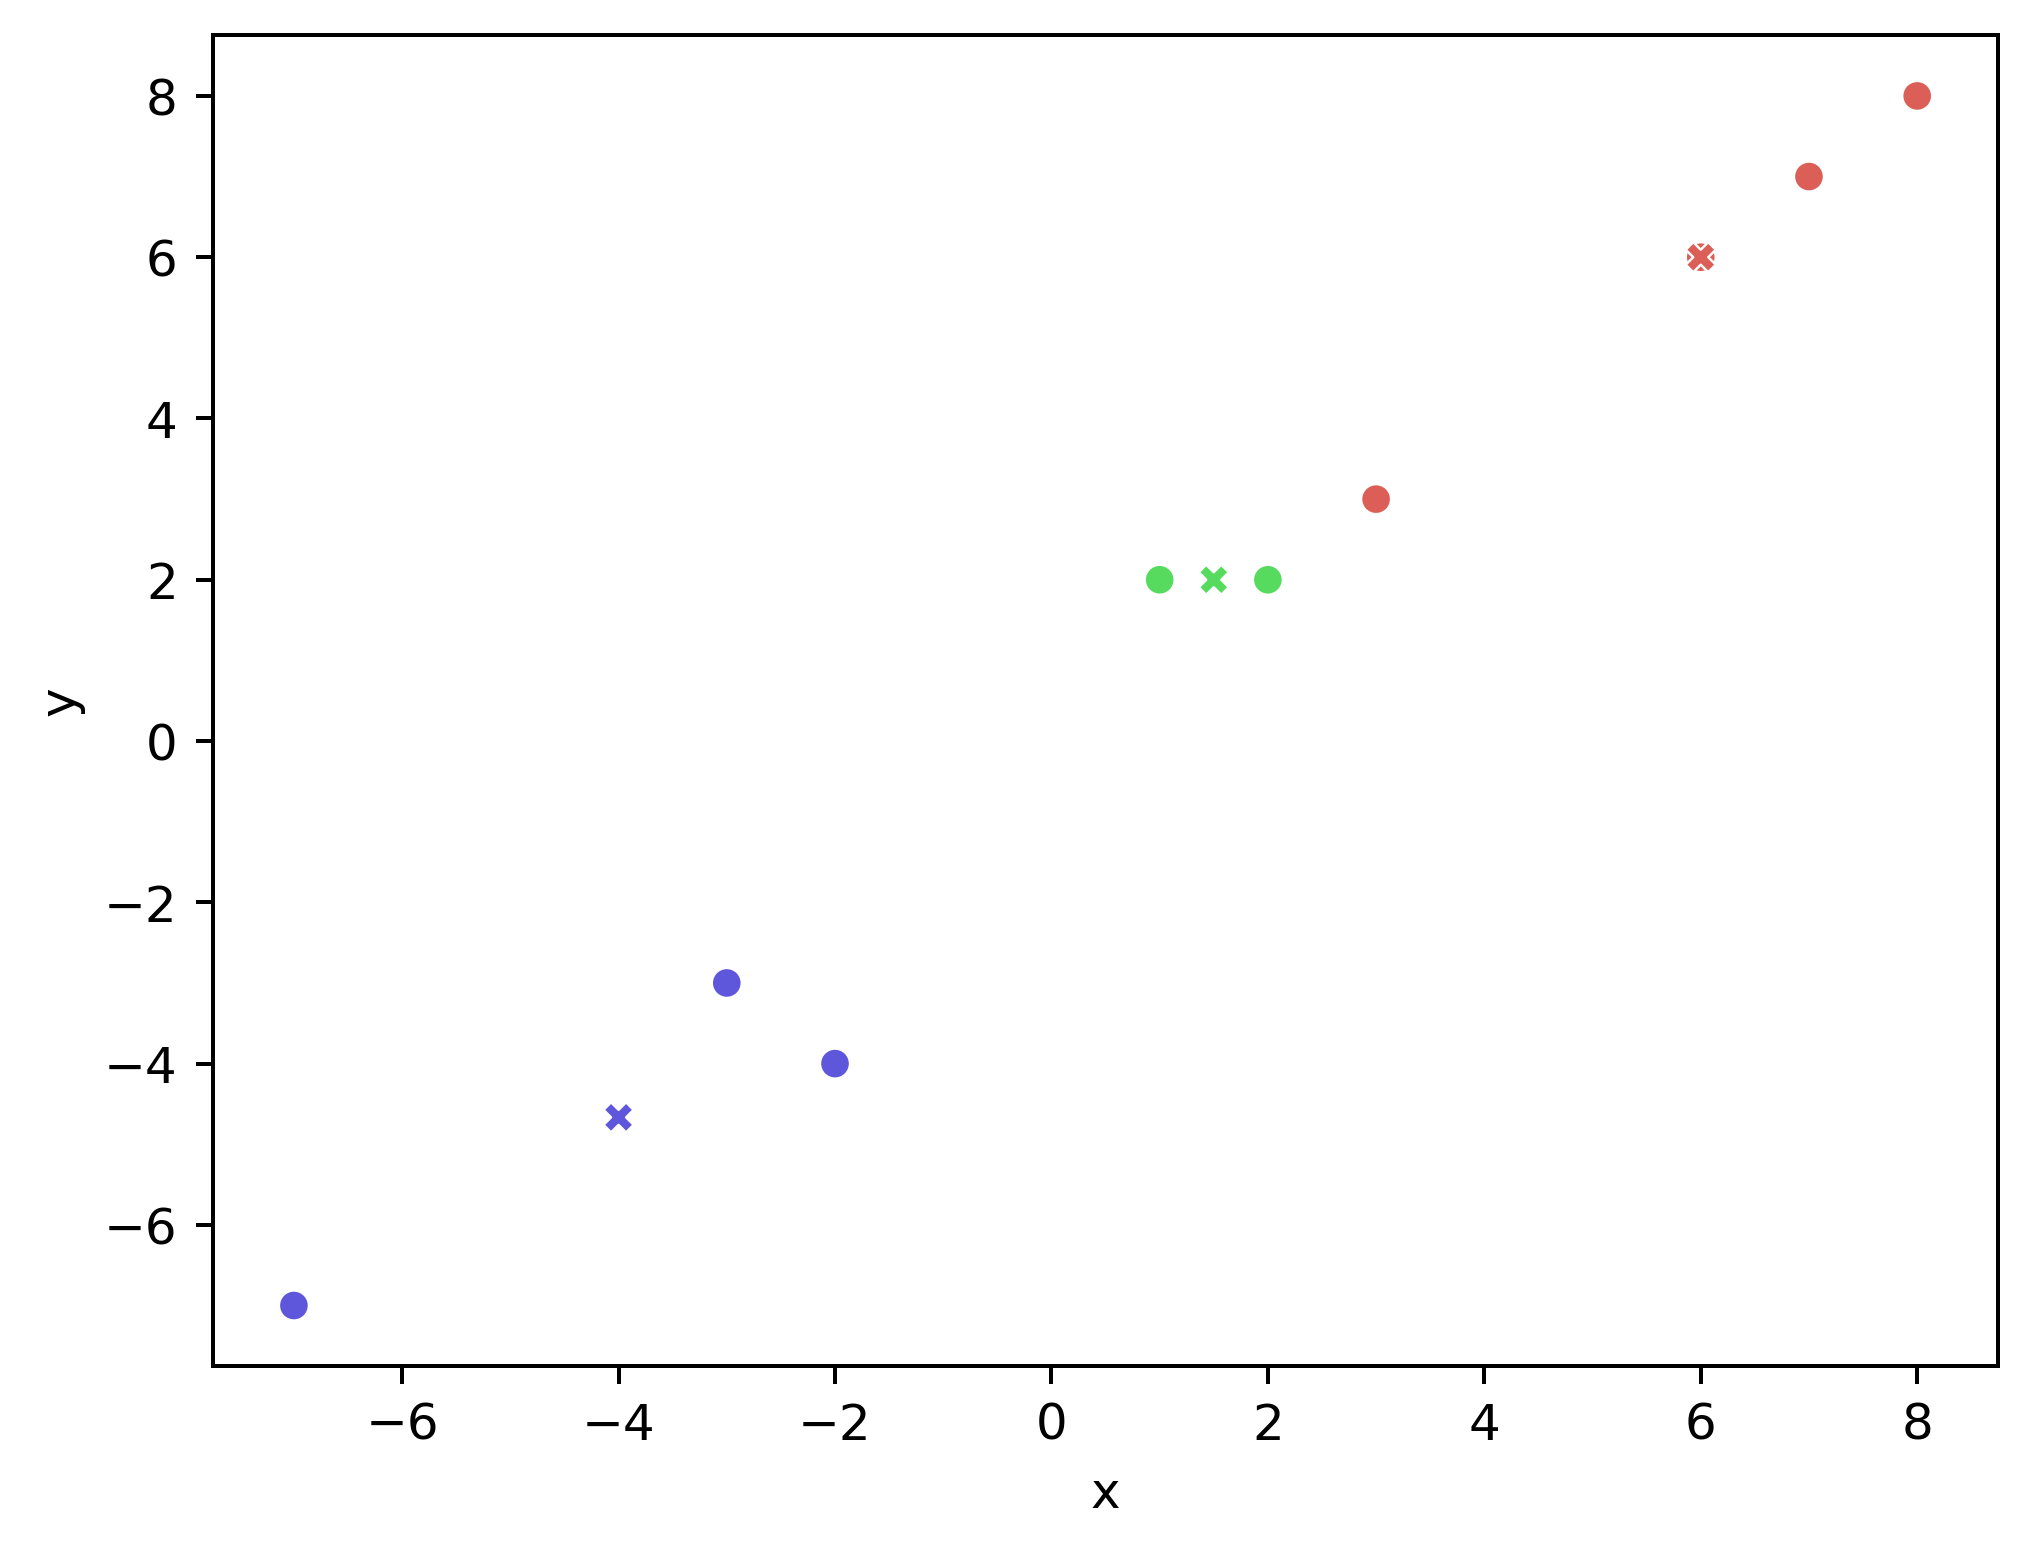
\includegraphics[width=0.5\textwidth]{img/kmean00.png}
    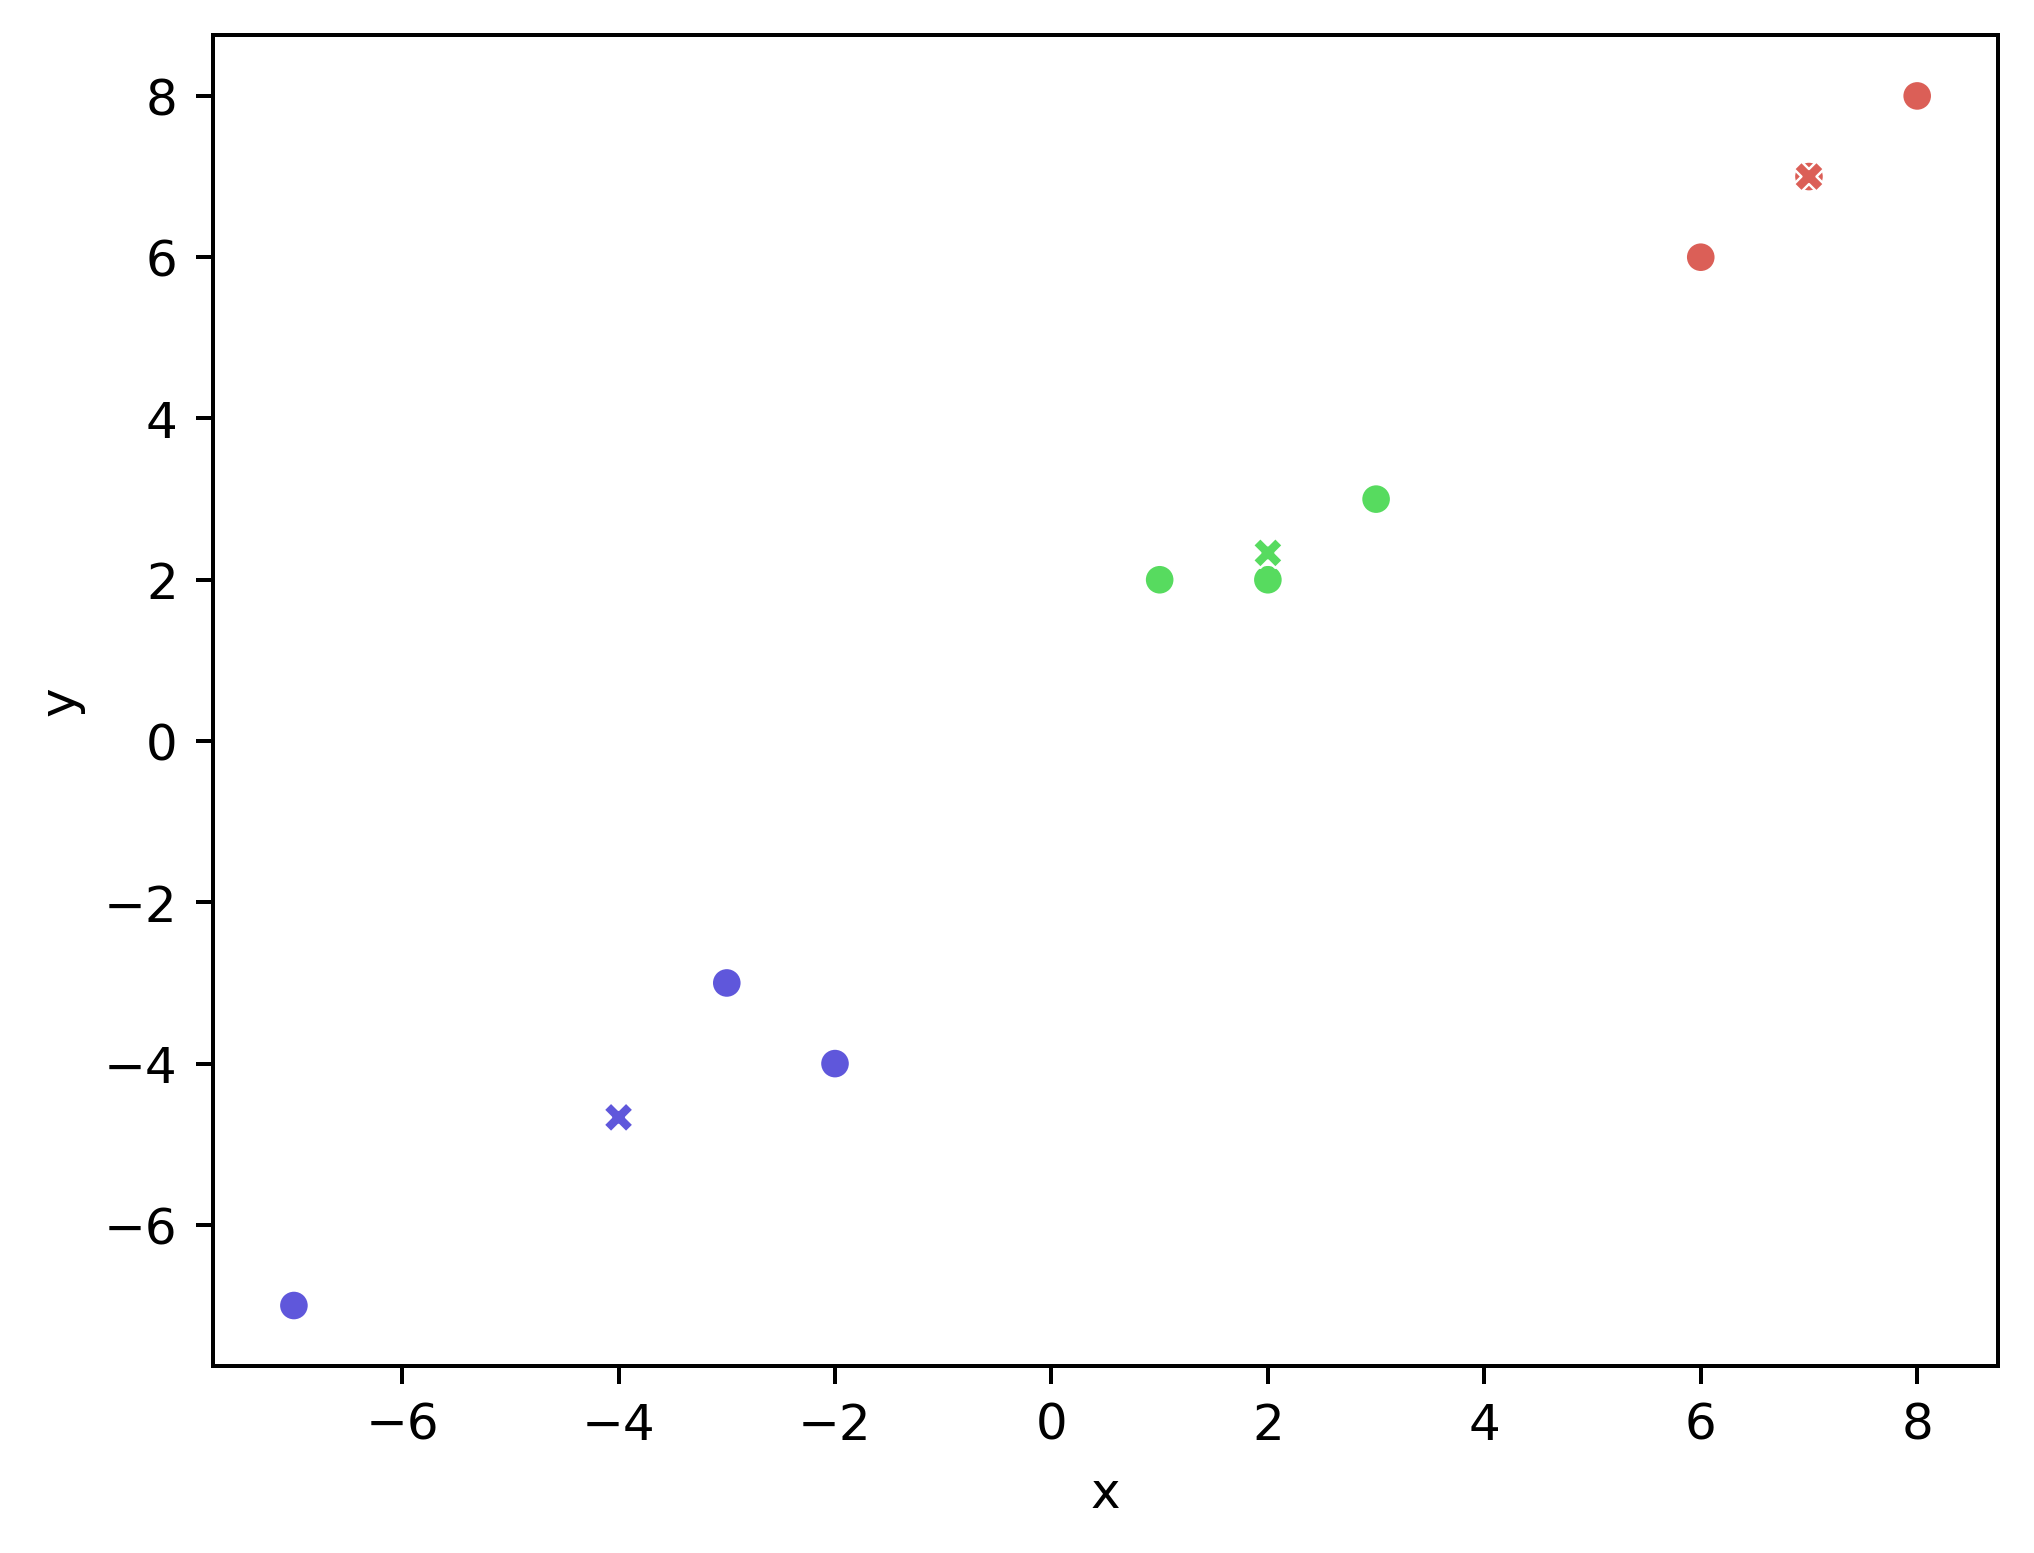
\includegraphics[width=0.5\textwidth]{img/kmean01.png}
\end{center}
\question{If the starting points are (-3,-3), (2,2), and (-7,-7), what happens?}
The algorithm completes in one iteration. The points are assigned as follows:
\begin{center}
    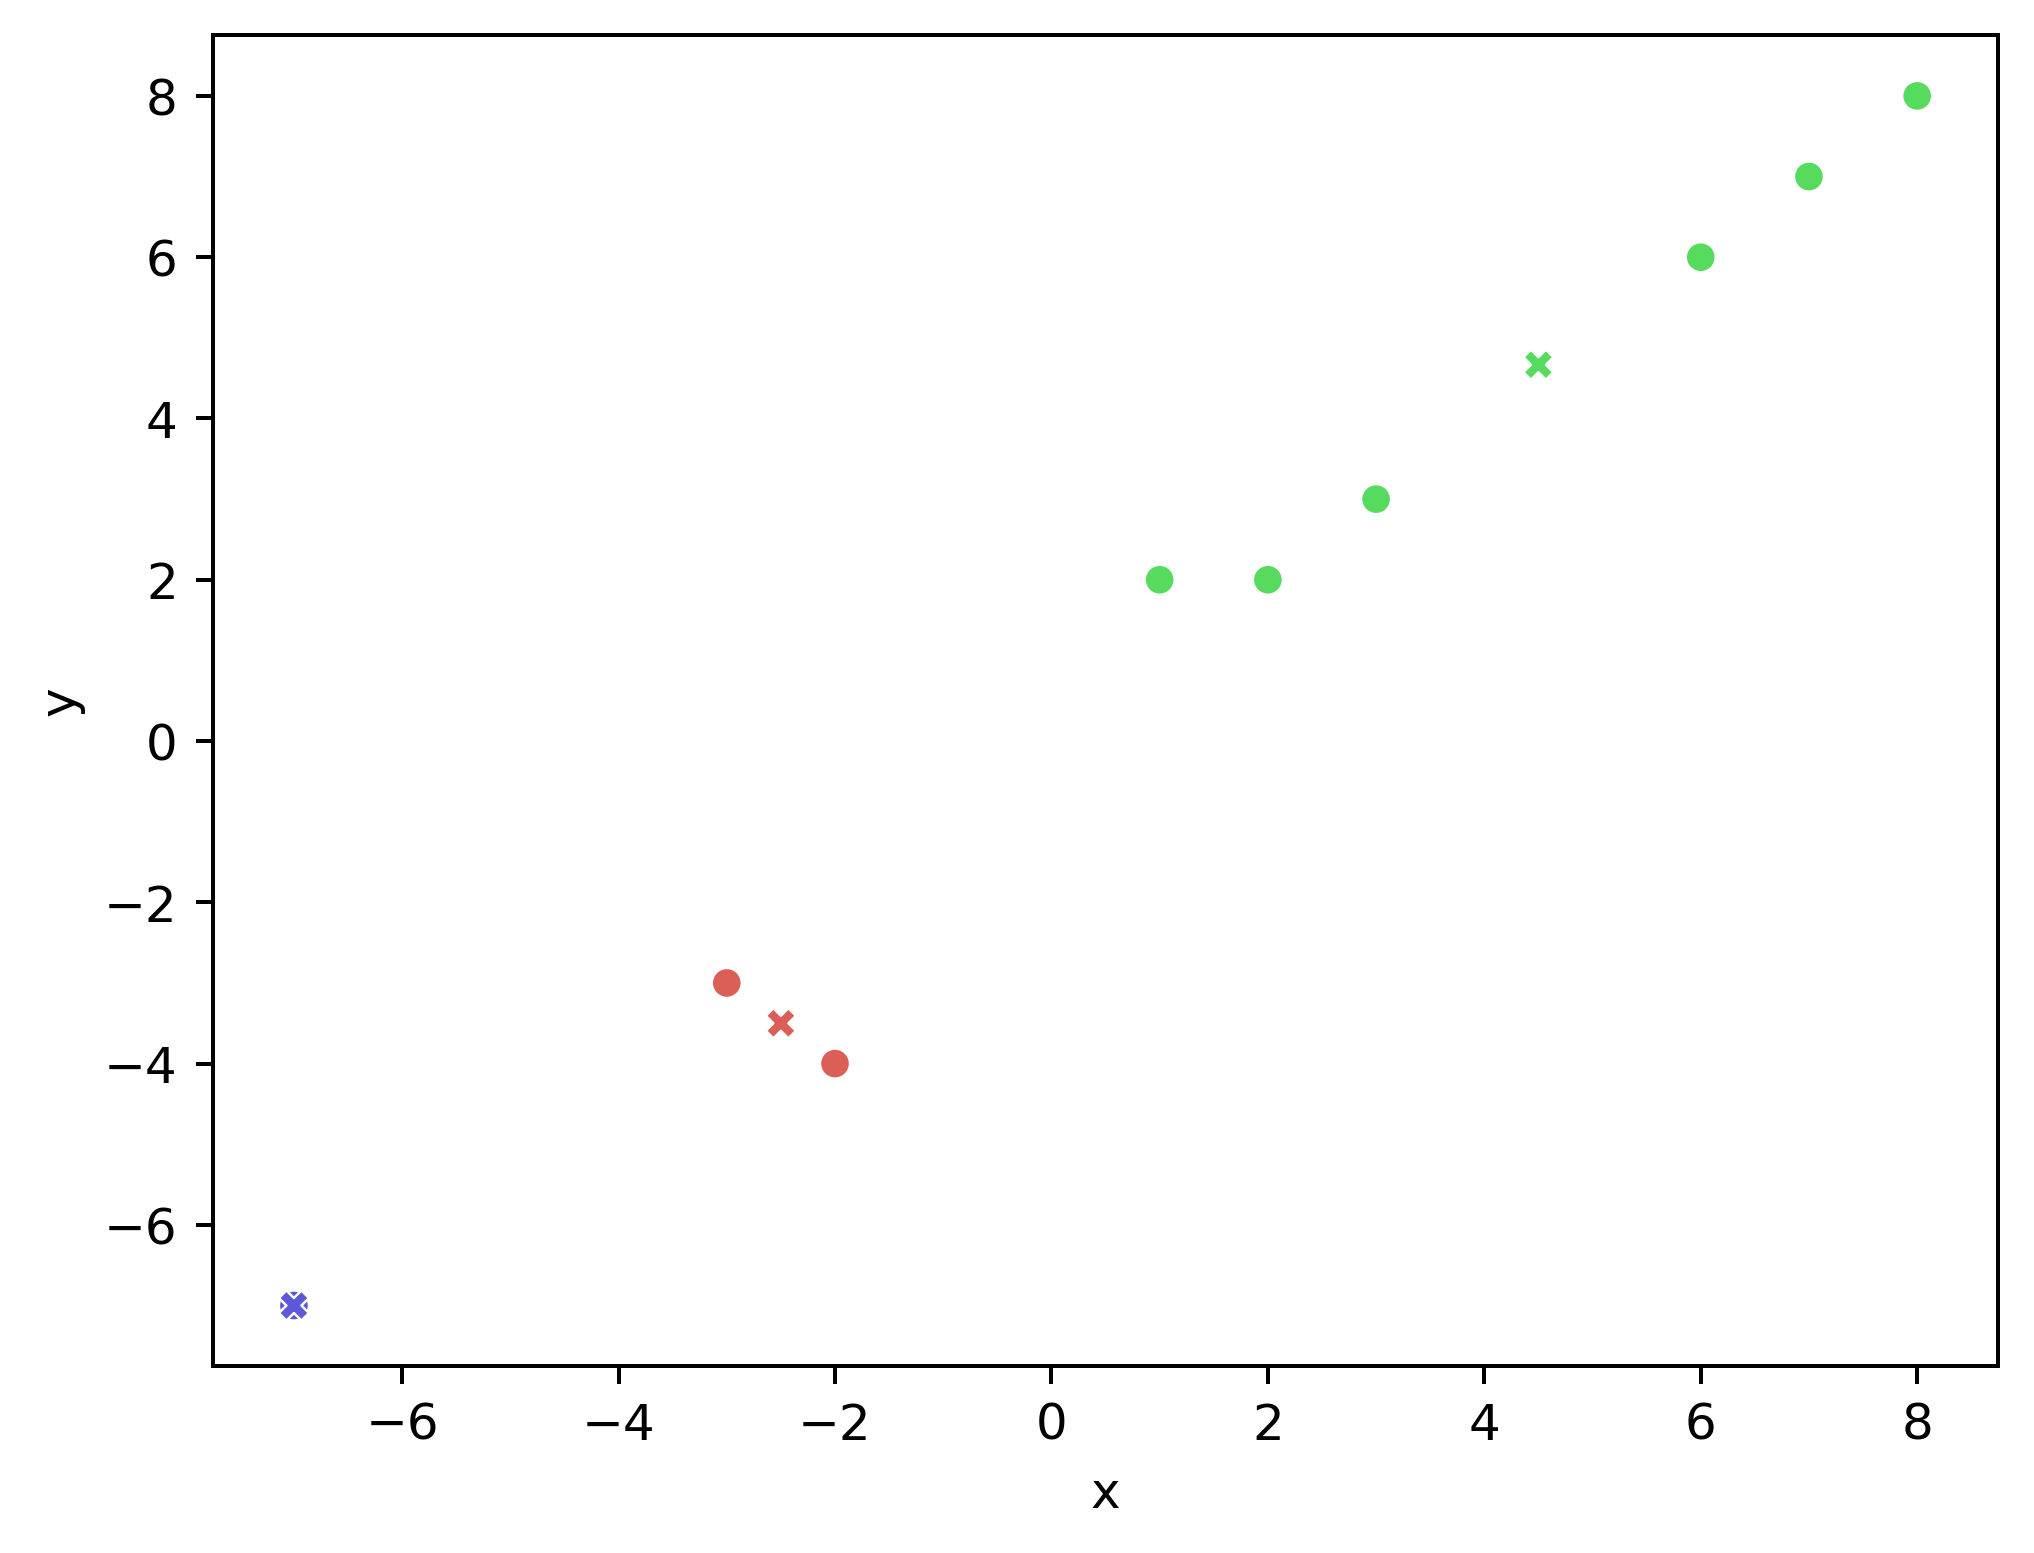
\includegraphics[width=0.5\textwidth]{img/kmean10.png}
\end{center}
\question{Between the two starting set of points in the previous two questions,
    which one do you think is better? How would you measure the `goodness' quality
    of a set of starting points?}
The first starting point results in a better clustering. The goodness of clusters could be measureed by
sum of squared error of point in each group to its centroid.
\extraquestion{What would be the best K for this question? Describe your reasoning.}
By inspection, the best K for this question should be 4. Since the data seems to be clustered into 4 distinct groups from lower left to upper right.
\subsection*{My heart will go on}
\question{What is the median age of the training set?}
28
\question{Some fields like `Embarked' are categorical. They need to be converted
    to numbers first. We will represent S with 0, C with 1, and Q with 2. What is
    the mode of Embarked? Do the same for Sex.}
The mode of Embarked is S. The mode of Sex is male.
\question{Write a logistic regression classifier using gradient descent as learned
    in class. Use PClass, Sex, Age, and Embarked as input features.}
See the submitted Jupyter Notebook.
\question{Submit a screenshot of your submission (with the scores). Upload
    your code to courseville.}
\begin{center}
    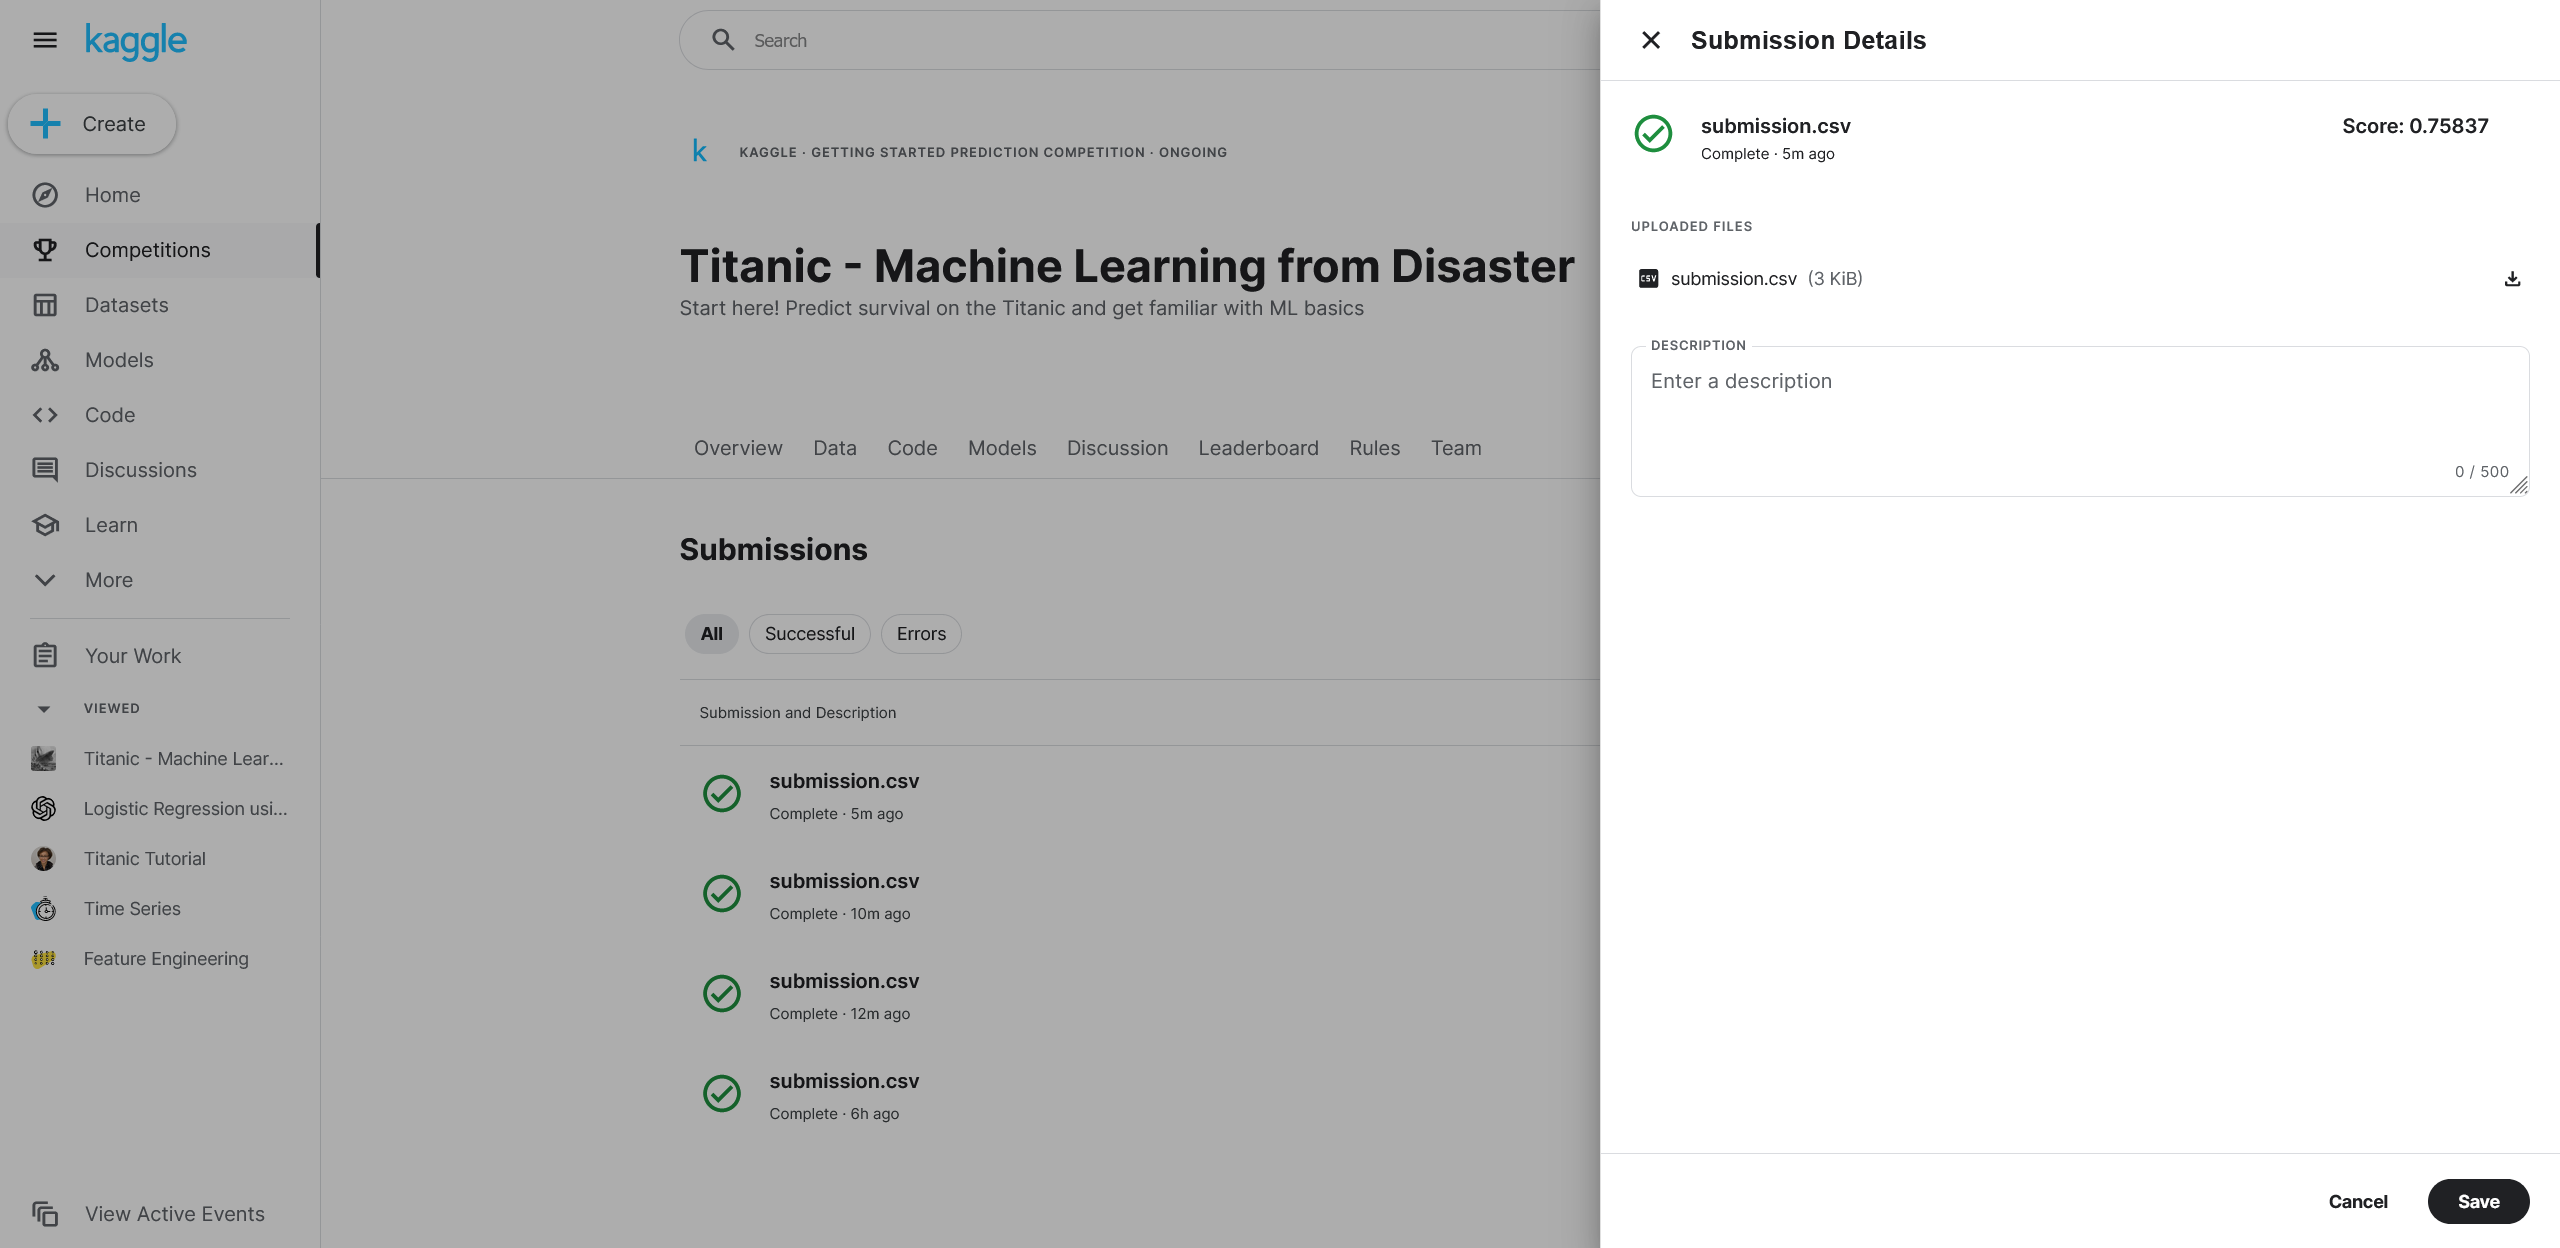
\includegraphics[width=0.8\textwidth]{img/submission1.png}
\end{center}
\question{Try adding some higher order features to your training (\(x_1^2\), \(x_1 x_2\), ...).
    Does this model has better accuracy on the training set? How does it
    perform on the test set?}
The model has better accuracy on the training set but worse on the test set. (0.79574 and 0.76794 respectively)
\question{What happens if you reduce the amount of features to just Sex and Age?}
The model has around 76.56\% accuracy on the test set.
\extraquestion{We want to show that matrix inversion yields the same answer
    as the gradient descent method. However, there is no closed form solution for
    logistic regression. Thus, we will use normal linear regression instead. Redo
    the Titanic task as a regression problem by using linear regression. Use the
    gradient descent method.}
See the submitted Jupyter Notebook.
\extraquestion{Now try using matrix inversion instead. However Are the weights
    learned from the two methods similar? Report the Mean Squared Errors (MSE)
    of the difference between the two weights.}
The weight from gradient descent is
\begin{center}
    \begin{verbatim}
    array([-0.18547017, -0.48995304, -0.004888, 0.04964349, 1.25428927])
    \end{verbatim}
\end{center}
The weight from matrix inversion is
\begin{center}
    \begin{verbatim}
    array([-0.18843944, -0.49086711, -0.00505436, 0.04911346, 1.26741154])
    \end{verbatim}
\end{center}
The MSE of gradient descent and matrix inversion are \(0.14493405967717804\) and
\(0.1449257376613481\) respectively.

The weights and MSE are similar. With an appropriate choice of learning rate, and number of epochs, the gradient descent parameters will converge to those of matrix inversion.
% \subsection*{Fun with matrix algebra}
% Prove the following statements.
% \extraquestion{\(\nabla_A tr AB = B^T\)}
% \extraquestion{\(\nabla_{A^T} f(A) = (\nabla_A f(A))^T\)}
% \extraquestion{\(\nabla_A tr ABA^TC = CAB+C^TAB^T\)}
\end{document}